\documentclass[12pt]{article}

\setlength\parindent{0pt}
\newcommand{\myt}[1]{\textbf{\underline{#1}}}

\usepackage{mathtools}
\usepackage{amssymb}
\usepackage{graphicx}

\title{\vspace{-15ex}Math 239 Lecture 23\vspace{-1ex}}
\date{July 3rd, 2015}
\author{Graham Cooper}

\begin{document}
	\maketitle
	Items:
	\begin{itemize}
		\item Trees
		\item Spanning Trees
	\end{itemize}
	
	\section*{Trees}
	Evrey tree qwith 22 vertices has 22 leaves\\
	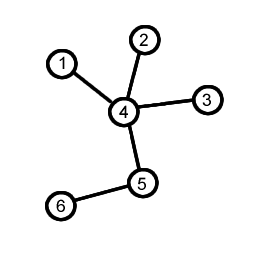
\includegraphics[scale=0.5]{tinytree.png}\\
	
	\myt{Theorem:} Every tree with n vertices has n-1 edges.\\
	
	\myt{Proof:} By induction on n.\\
	Base Case: When n = 1, there is only one tree with 1 vertex and that tree has n-1 = 0 edges\\
	
	Induction Hyptothesis: Assume every tree with n-1 vertices has n-2 edges.\\
	
	Induction Step: Let T be a tree with n vertices. Let v be a leaf of T and let e be the only edge incident wiht v. Remove e and v from T to get T'. When we remove e from T there are 2 components, one consists of only v and the other is T'. So T' is connected. Also, T' has no cycles since T has no cycles. So T' is a tree with n-1 vertices. By induction hypothese T' has n-2 edges, so T has n-1 edges\\
	
	\myt{Q}: How many edges does a forest with n vertices and k components have?
	
	\myt{A}: n-k, each component has one feqer edfe than vertices. $\implies$ k compnents mean k fewer edges in total\\
	
	\myt{Theorem:} There is a unique path between every pair of vertices in a tree\\
	
	\myt{Proof:} Suppose BWOC there are two u,v-paths P1, P2. There is an edge e=xy in one path but not the other. WLOG e $\in$ P1, P1 = e,v1,...,vk,x,y,vk+1,...v. Then x,vk,...,u,P2,V,...,vk+1, y is an x,y-walk not using e. So there is an x,y-path P3, without using e. Then P + e is a cycle in the tree, conradiction.
	
	\myt{Theorem:} A tree is bipartite\\
	\myt{Proof:} By induction!\\
	
	\section*{Spanning Trees}
	\myt{Definition:} T is a spanning tree of a graph G is T is a subgraph of G that is a tree and uses very vertex in G\\
	
	\myt{Definition:} Minimum Spanning Tree is a tree with the minimum total cost\\
	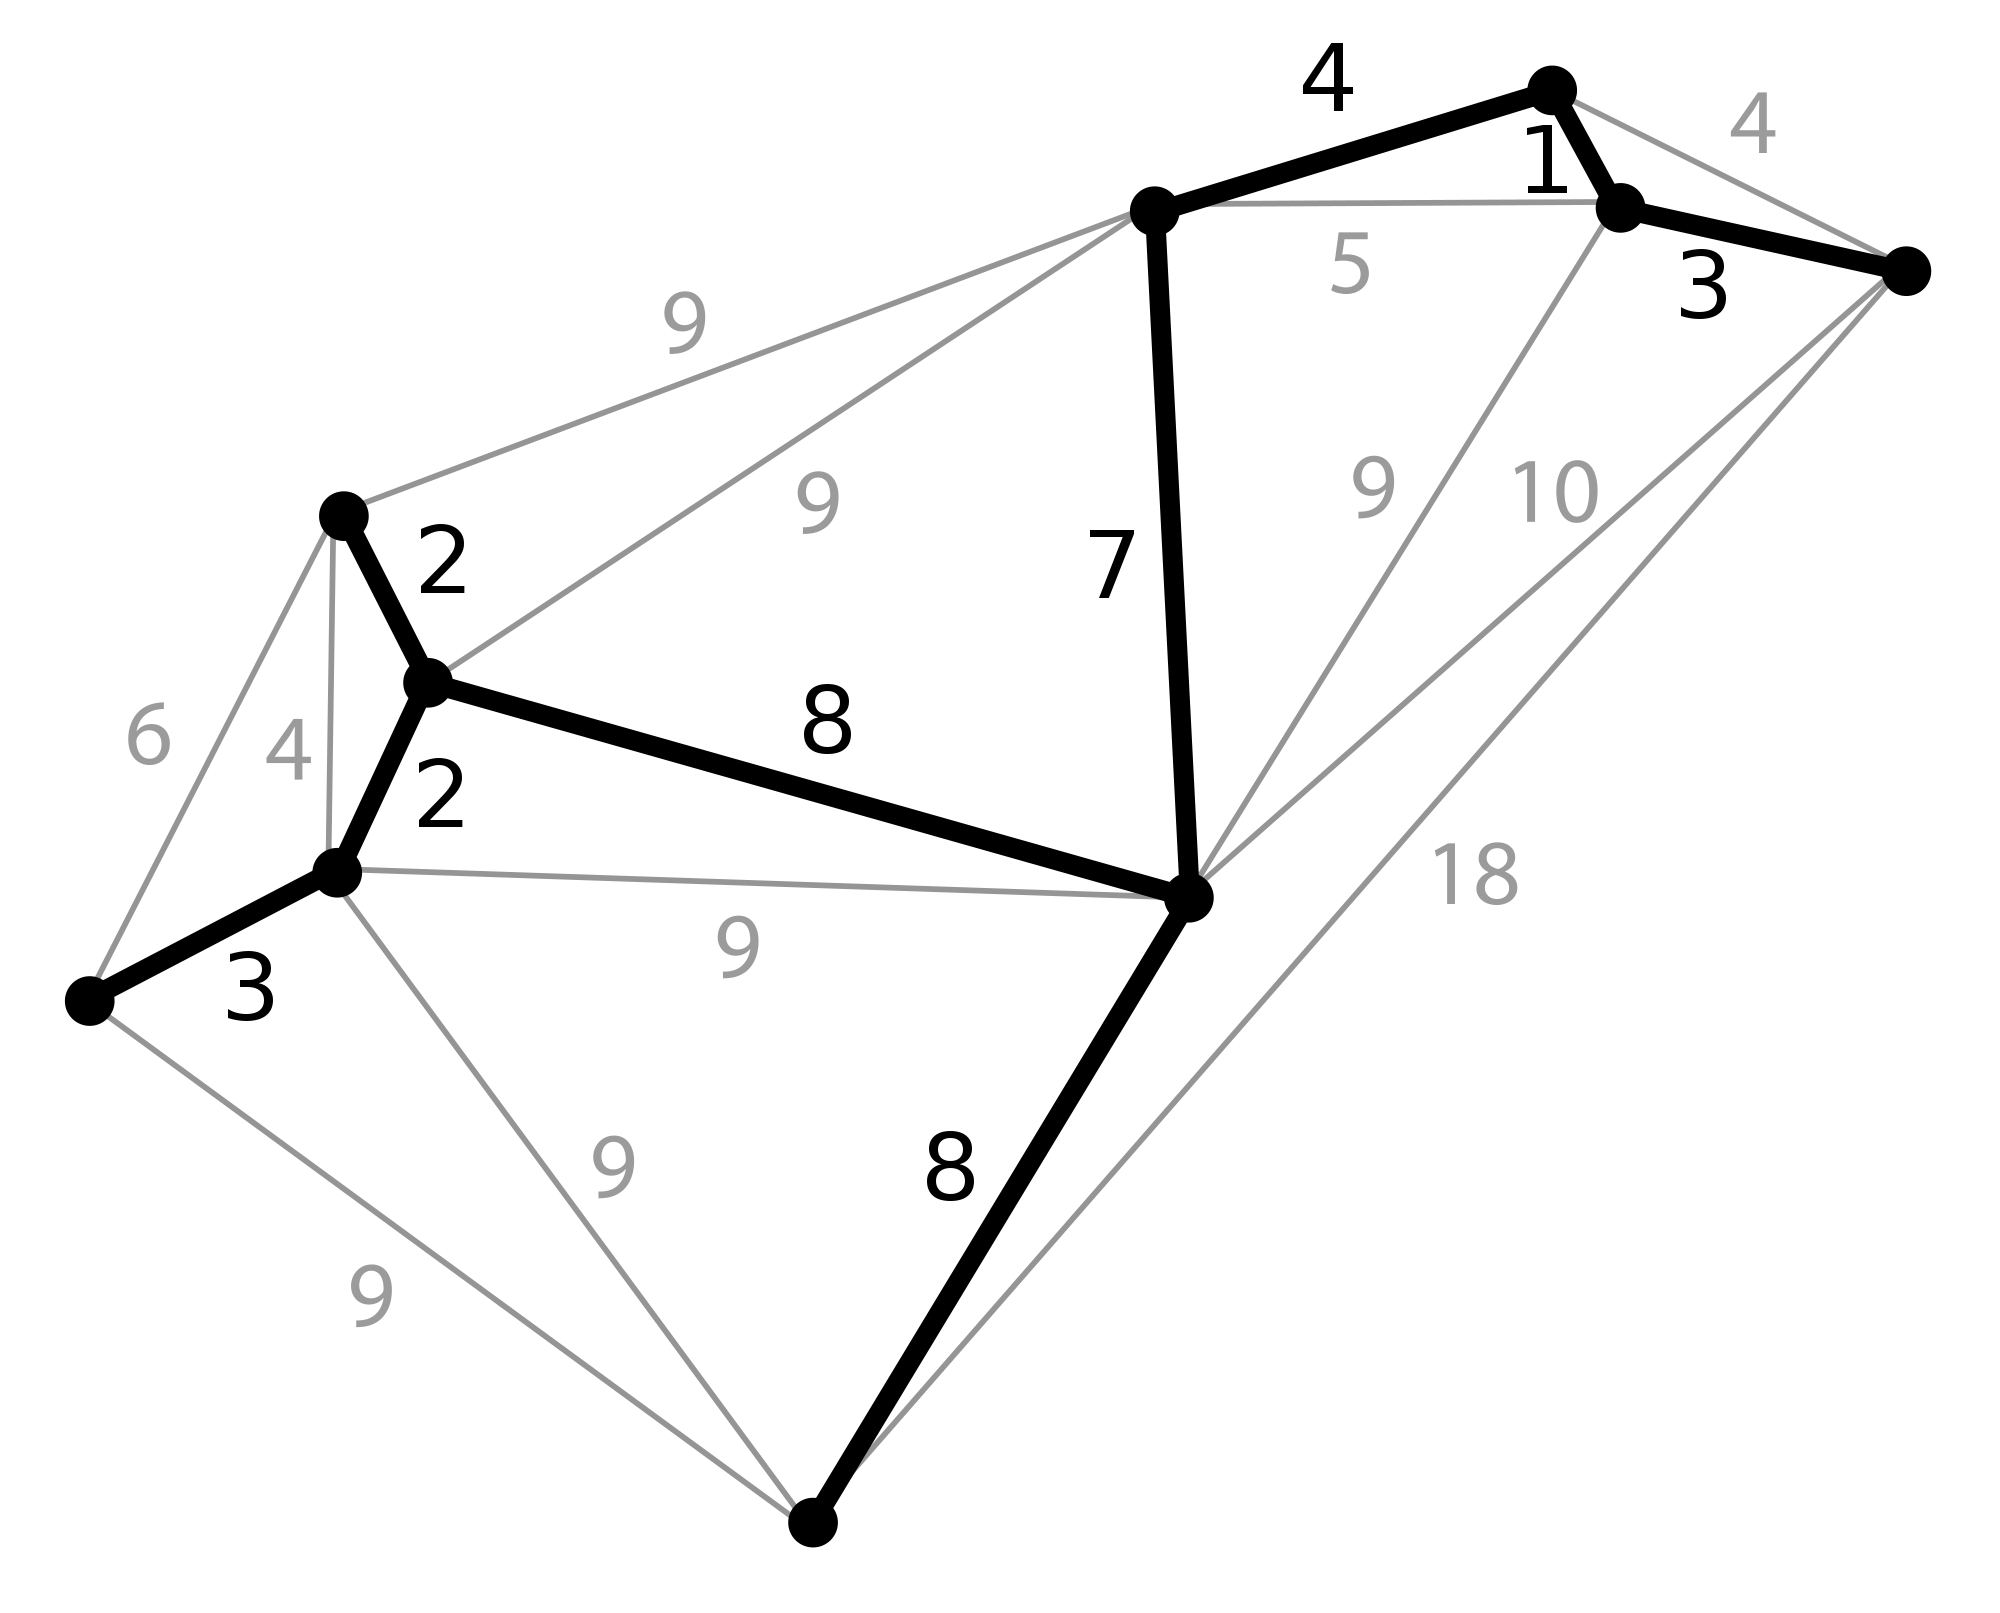
\includegraphics[scale=0.1]{spanningtree.png}\\
	
	\myt{Theorem:} A graph G is connected if and only if G contains a spanning tree\\
	\myt{Proof:} $\impliedby$ Suppose T is a spanning tree in G. For any u,v $\in$ V(G) there is a u,v-path in T, which is also in G. So G is connected\\
	$\implies$ Supose G is connected. Prove this by induction on the number of edges m in G with n vertices.\\
	Base case: When m=n-1, G is a tree, so it has a spanning tree.\\
	Induction hypothesis: Assume ny conneted graph with m-1 edges and n vertices has a spanning tree\\
	
	
\end{document}
